\documentclass[tikz,border=12pt]{standalone}
\usepackage{tikz}
\usetikzlibrary{positioning, arrows.meta, decorations.markings}

\definecolor{fast}{RGB}{60, 179, 113}
\definecolor{slow}{RGB}{218, 130, 50}

\begin{document}
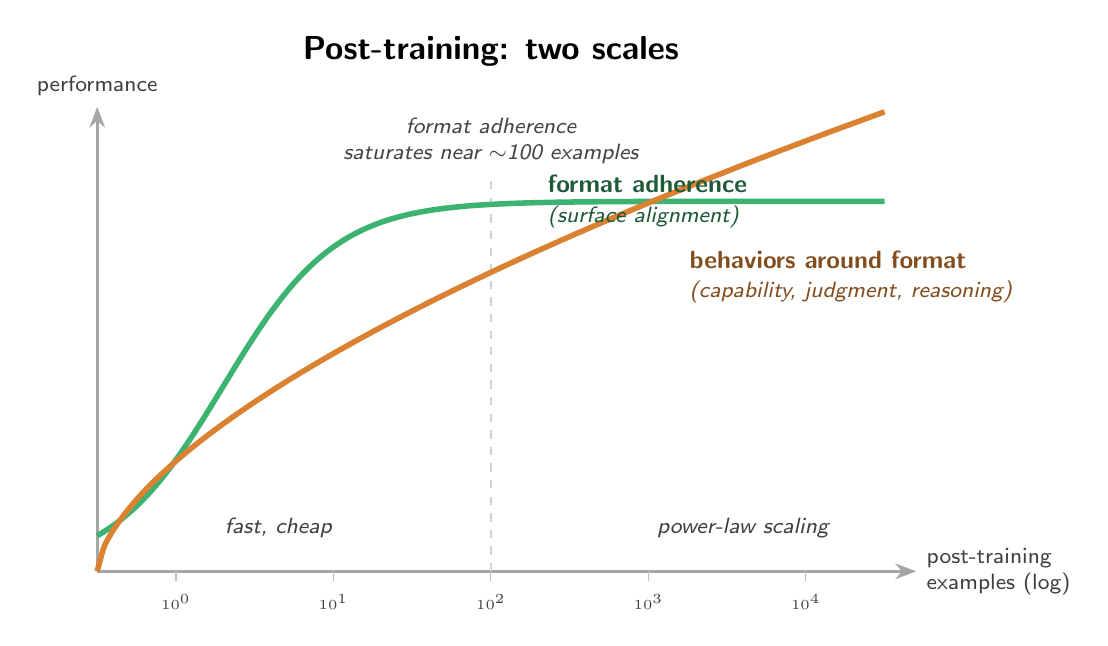
\begin{tikzpicture}[
    >=Stealth,
    font=\sffamily,
]

\def\xmax{10}
\def\ymax{5.5}

% --- Title ---
\node[font=\sffamily\large\bfseries]
    at (\xmax/2, \ymax+1.1) {Post-training: two scales};

% --- Axes ---
\draw[->, gray!70, line width=1pt]
    (0,0) -- (\xmax+0.4, 0)
    node[right, text=gray!50!black, font=\sffamily\footnotesize, align=left]
        {post-training\\examples (log)};
\draw[->, gray!70, line width=1pt]
    (0,0) -- (0, \ymax+0.4)
    node[above, text=gray!50!black, font=\sffamily\footnotesize] {performance};

% --- Log-scale x-axis ticks ---
\foreach \x/\lbl in {1/{$10^0$}, 3/{$10^1$}, 5/{$10^2$}, 7/{$10^3$}, 9/{$10^4$}} {
    \draw[gray!50] (\x,0) -- (\x,-0.12);
    \node[below=2pt, font=\sffamily\tiny, text=gray!50!black] at (\x,-0.1) {\lbl};
}

% --- Saturation marker (vertical guide at ~100 examples) ---
\draw[gray!35, dashed, line width=0.9pt] (5, 0) -- (5, 5.0);
\node[font=\sffamily\footnotesize\itshape, text=gray!55!black,
      align=center, anchor=south]
    at (5, 5.05) {format adherence\\saturates near $\sim$100 examples};

% --- Format adherence curve (sigmoid; saturates near x = 4) ---
\draw[fast, line width=2pt, smooth, samples=120, domain=0:\xmax]
    plot (\x, {4.7 / (1 + exp(-1.4*(\x - 1.6)))});

% --- Capability / behaviors-around-format curve (power-law-ish, keeps rising) ---
\draw[slow, line width=2pt, smooth, samples=120, domain=0:\xmax]
    plot (\x, {1.4 * pow(\x, 0.62)});

% --- Curve labels ---
\node[fast!50!black, font=\sffamily\small\bfseries, anchor=west]
    at (5.6, 4.92) {format adherence};
\node[fast!50!black, font=\sffamily\footnotesize\itshape, anchor=west]
    at (5.6, 4.50) {(surface alignment)};

\node[slow!60!black, font=\sffamily\small\bfseries, anchor=west]
    at (7.4, 3.95) {behaviors around format};
\node[slow!60!black, font=\sffamily\footnotesize\itshape, anchor=west]
    at (7.4, 3.55) {(capability, judgment, reasoning)};

% --- Region annotations ---
\node[font=\sffamily\footnotesize\itshape, text=gray!50!black,
      align=center]
    at (2.3, 0.55) {fast, cheap};
\node[font=\sffamily\footnotesize\itshape, text=gray!50!black,
      align=center]
    at (8.2, 0.55) {power-law scaling};

\end{tikzpicture}
\end{document}
